\documentclass{article}

\usepackage{graphicx}
\usepackage{rotating}
\usepackage{amsmath}
\usepackage{amssymb}
\usepackage{fancyhdr}
\usepackage{listings}
\usepackage{lscape}
\usepackage{multirow}
\usepackage{color}
\usepackage{amsfonts}
\usepackage{textcomp}
\usepackage{float}
\usepackage{longtable}
\usepackage{booktabs}
\usepackage[sorting=none]{biblatex}
\usepackage[margin=1in]{geometry}
\usepackage[font={small,it}]{caption}
\usepackage[table,xcdraw]{xcolor}
\usepackage{placeins}
\usepackage{breqn}
\usepackage{xepersian}





%\DeclareMathOperator*{\btie}{\bowtie}
\addbibresource{bibliography.bib}
\settextfont[Scale=1.2]{B-NAZANIN.TTF}
\setlatintextfont[Scale=1]{Times New Roman}
\renewcommand{\baselinestretch}{1.5}
\pagestyle{fancy}
\fancyhf{}
\rhead{تکلیف اول درس آزمون نرم افزار}
\lhead{\thepage}
\rfoot{علیرضا ابره فروش}
\lfoot{9816603}
\renewcommand{\headrulewidth}{1pt}
\renewcommand{\footrulewidth}{1pt}
%%%%%%%%%%
\lstset
{
    language=[latex]tex,
    basicstyle=\ttfamily,
    commentstyle=\color{black},
    columns=fullflexible,
    keepspaces=true,
    upquote=true,
    showstringspaces=false,
    morestring=[s]\\\%,
    stringstyle=\color{black},
}
%%%%%%%%%%
%beginMatlab
\definecolor{mygreen}{RGB}{28,172,0} % color values Red, Green, Blue
\definecolor{mylilas}{RGB}{170,55,241}
%endMatlab
\begin{document}
%beginMatlab
\lstset{language=Matlab,%
    %basicstyle=\color{red},
    breaklines=true,%
    morekeywords={matlab2tikz},
    keywordstyle=\color{blue},%
    morekeywords=[2]{1}, keywordstyle=[2]{\color{black}},
    identifierstyle=\color{black},%
    stringstyle=\color{mylilas},
    commentstyle=\color{mygreen},%
    showstringspaces=false,%without this there will be a symbol in the places where there is a space
    numbers=left,%
    numberstyle={\tiny \color{black}},% size of the numbers
    numbersep=9pt, % this defines how far the numbers are from the text
    emph=[1]{for,end,break},emphstyle=[1]\color{red}, %some words to emphasise
    %emph=[2]{word1,word2}, emphstyle=[2]{style},    
}
%endMatlab
\begin{titlepage}
\begin{center}

\includegraphics[width=0.4\textwidth]{figures/IUT Logo.png}\\
        
\LARGE
\textbf{دانشگاه صنعتی اصفهان}\\
\textbf{دانشکده مهندسی برق و کامپیوتر}\\
        
\vfill
        
\huge
\textbf{عنوان: تکلیف چهارم درس ریزپردازنده}\\
        
\vfill
        
\LARGE
\textbf{نام و نام خانوادگی: علیرضا ابره فروش}\\
\textbf{شماره دانشجویی: 9816603}\\
\textbf{نیم\,سال تحصیلی: پاییز 1400}\\
\textbf{مدرّس: دکتر عارف کریمی افشار}\\
\end{center}
\end{titlepage}


%\tableofcontents
\newpage

\section{}%1
\subsection{سوال 3 فصل ششم}
\subsubsection{\lr{a}}
\begin{figure}[H]
    \centering
    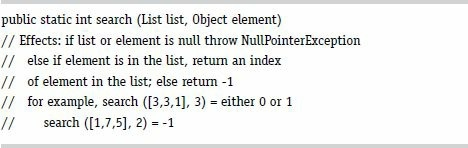
\includegraphics[width=1.0\textwidth]{figures/1a.jpg}
    \caption
	{}
    \label{fig:fig1}
\end{figure}
\begin{figure}[H]
    \centering
    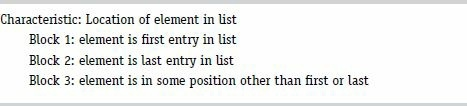
\includegraphics[width=1.0\textwidth]{figures/1b.jpg}
    \caption
	{}
    \label{fig:fig1}
\end{figure}
اگر لیست ما تک عضوی باشد، برای مثال $\left\{ apple \right\}$ و عنصر مورد جستجوی ما \lr{apple} باشد، این عنصر در هر دو بلاک می‌تواند قرار گیرد. پس ویژگی \lr{“Location of element in list”} نمی‌تواند تهی بودن اشتراک بین هر دو بلاک را حفظ کند و در نتیجه فضای ورودی را به درستی افراز کند.

\subsubsection{\lr{b}}
اگر عنصر در لیست وجود نداشته باشد هیچ بلاکی این حالت را در نظر نمی‌گیرد. برای مثال $\left\{ apple, orange, banana \right\}$ و عنصر مورد جستجو $melon$ باشد، هیچ یک از سه بلاک بالا این حالت را پوشش نمی‌دهند.

\subsubsection{\lr{c}}
\begin{latin}
\begin{table}[H]
\begin{tabular}{|l|c|c|}
\hline
                                                                                          & \textbf{Block: 1} & \textbf{Block: 2} \\ \hline
\textbf{Characteristic: element is the first entry in list}                                 & True        & False       \\ \hline
\textbf{Characteristic: element is the last entry in list}                                  & True        & False       \\ \hline
\textbf{Characteristic: element is neither first nor last in the list but is in the list} & True        & False       \\ \hline
\textbf{Characteristic: element is not in the list}                                       & True        & False       \\ \hline
\end{tabular}
\end{table}
\end{latin}

\subsection{سوال 4 فصل ششم}
جهت افراز فضای ورودی برای کلاس \texttt{GenericStack} می‌توانیم ‌افرازها و بلوک‌های زیر در نظر بگیریم:
\begin{latin}
1. \texttt{GenericStack()} constructor:
   \begin{itemize}
   \item Partition 1: Empty stack creation
   \item Partition 2: Stack creation with initial capacity
   \item Partition 3: Stack creation with initial capacity less than 1
   \item Partition 4: Stack creation with null initial capacity
   \end{itemize}
2. \texttt{push(Object X)} method:
   \begin{itemize}
   \item Partition 1: Pushing a non-null object onto an empty stack
   \item Partition 2: Pushing a non-null object onto a non-empty stack
   \item Partition 3: Pushing a null object onto an empty stack
   \item Partition 4: Pushing a null object onto a non-empty stack
   \end{itemize}
3. \texttt{pop()} method:
   \begin{itemize}
   \item Partition 1: Popping from an empty stack
   \item Partition 2: Popping from a non-empty stack
   \end{itemize}
4. \texttt{isEmpty()} method:
   \begin{itemize}
   \item Partition 1: Calling \texttt{isEmpty()} on an empty stack
   \item Partition 2: Calling \texttt{isEmpty()} on a non-empty stack
   \end{itemize}
\end{latin}
این تقسیم‌بندی‌ها فضای ورودی را به سناریوهای خاص تقسیم می‌کنند که جوانب مختلف کلاس \texttt{GenericStack} را پوشش می‌دهند. با انتخاب ورودی‌های آزمون از این تقسیم‌بندی‌ها، می‌توانیم پوشش مناسبی از قابلیت‌های ارائه شده توسط این کلاس را به دست آوریم.

\begin{latin}
\subsubsection{a}
The input variables for the GenericStack class are:
\begin{itemize}
\item \textbf{X}: The object to be pushed onto the stack.
\end{itemize}

The state variables are:
\begin{itemize}
    \item \textbf{Stack}: The data structure used to store the elements in the stack.
\end{itemize}

\subsubsection{b}
Characteristics of the input variables:
\begin{itemize}
    \item \textbf{X}:
    \begin{itemize}
        \item Type: Object
        \item Valid values: Any object, including null
    \end{itemize}
\end{itemize}

\subsubsection{c}
Characteristics of inputs:
\begin{itemize}
    \item \textbf{Stack size}:
    \begin{itemize}
        \item Type: Integer
        \item Range: Non-negative integers (including zero)
        \item Invalid values: Negative values
    \end{itemize}
\end{itemize}

\subsubsection{d}
Partitioning the characteristics into blocks:
\begin{itemize}
    \item Partition 1: \textbf{Stack size}
    \begin{itemize}
        \item Block 1 (\textit{Base}): Zero size
        \item Block 2: Non-zero size
    \end{itemize}
\end{itemize}

\subsubsection{e}
Values for each block:
\begin{itemize}
    \item Block 1 (\textit{Stack size}):
    \begin{itemize}
        \item \textit{Base}: size = 0
    \end{itemize}
    
    \item Block 2 (\textit{Stack size}):
    \begin{itemize}
        \item \textit{Base}: size = 1
        \item Additional: size = 2
    \end{itemize}
\end{itemize}

\end{latin}



\section{}%2
\subsection{سوال 4 فصل ششم صفحه‌ی 139}
\subsubsection{\lr{a}}
بله شرط \lr{Completeness} را ارضا می‌کند. چون هر ورودی در یکی از سه حالت مذکور دسته‌بندی می‌شود.
\subsubsection{\lr{b}}
بله شرط \lr{Disjointness} را ارضا می‌کند.
\subsubsection{\lr{c}}
بله شرط \lr{Completeness} را ارضا می‌کند.
\subsubsection{\lr{d}}
خیر اگر $S_1$ و $S_2$ تهی باشند در هر چهار بلاک دسته‌بندی می‌شوند. پس شرط \lr{Disjointness} را حفظ نمی‌کند.
\subsubsection{\lr{e}}
\begin{latin}
$1 + \sum_{i = 1}^{Q} \left( B_i - 1 \right) = 1 + (3 - 1) + (4 - 1) = 1 + 2 + 3 = 6$
\end{latin}
\subsubsection{\lr{f}}
\begin{latin}
Characteristic: relation between s1 and s2
   \begin{itemize}
   \item s1 and s2 represent the same non-empty set
   \item s1 is a non-empty subset of s2
   \item s2 is a non-empty subset of s1
   \item s1 and s2 do not have any elements in common (one or both could be empty)
   \end{itemize}
\end{latin}

\subsection{سوال 5 فصل ششم صفحه‌ی 139}
\subsubsection{\lr{a}}
\begin{latin}
$\left( Value 1, Value 2, Operation \right) \in  \left\{ \left( -1, -1, '+' \right), \left( 0, 0, '-' \right), \left( 1, 1, '\times' \right), \left( -1, 2, '\div' \right) \right\}$
\end{latin}
\subsubsection{\lr{b}}
\begin{latin}
$\text{Base choice: } Value 1 \ge 0, Value 2 \ge 0, Operation = '+' \\
\left( Value 1, Value 2, Operation \right) \in \left\{ 
\left( 1, 1, '-' \right),
\left( 1, 1, '\times' \right),
\left( 1, 1, '\div' \right),
\left( 1, 0, '+' \right),
\left( 1, -1, '+' \right),
\left( -1, 1, '+' \right),
\left( 0, 1, '+' \right)
 \right\}$
\end{latin}
\subsubsection{\lr{c}}
\begin{latin}
$3 \times 3 \times 4 = 36$
\end{latin}
\subsubsection{\lr{d}}
(لطفا زوم کنید :))\\
\resizebox{.9\hsize}{!}
{$
\left( Value 1, Value 2, Operation \right) \in \left\{ 
\left( -1, -1, '+' \right),
\left( -1, 0, '-' \right),
\left( -1, 1, '\times' \right),
\left( -1, -1, '\div' \right),
\left( 0, 0, '+' \right),
\left( 0, 1, '-' \right),
\left( 0, -1, '\times' \right),
\left( 0, 0, '\div' \right),
\left( 1, 1, '+' \right),
\left( 1, -1, '-' \right),
\left( 1, 0, '\times' \right),
\left( 1, 1, '\div' \right)
\right\}
$}


\section{}%3
(لطفا زوم کنید :))\\
\resizebox{.9\hsize}{!}
{$
\left( \max_{i = 1} ^ Q (B_i) \right) \times \left( \max_{j = 1, j \neq i} ^ Q (B_j) \right) = 4 \times 4 = 16 \\
\left\{
(A1, B1, C1, D1), (A1, B2, C2, D2), (A1, B3, C3, D3), (A1, B4, C4, D4),
(A2, B1, C2, D3), (A2, B2, C3, D4), (A2, B3, C4, D1), (A2, B4, C1, D2),
(A3, B1, C3, D1), (A3, B2, C4, D2), (A3, B3, C1, D3), (A3, B4, C2, D4),
(A4, B1, C4, D3), (A4, B2, C1, D4), (A4, B3, C2, D1), (A4, B4, C3, D2)
\right\}
$}



\section{}%4
\begin{latin}
\subsection{a}
The input variables for the BoundedQueue class are:
\begin{itemize}
\item \textbf{capacity}: The maximum number of elements allowed in the queue.
\item \textbf{X}: The object to be enqueued.
\end{itemize}
The state variables are:
\begin{itemize}
    \item \textbf{Queue}: The array or data structure used to store the elements in the queue.
    \item \textbf{Size}: The current number of elements in the queue.
    \item \textbf{Front}: The index of the front element in the queue.
    \item \textbf{Rear}: The index of the rear element in the queue.
\end{itemize}

\subsection{b}
Characteristics of the input variables:
\begin{itemize}
    \item \textbf{capacity}:
    \begin{itemize}
        \item Type: Integer
        \item Range: Positive integers (greater than zero)
        \item Invalid values: Negative values, zero
    \end{itemize}
    
    \item \textbf{X}:
    \begin{itemize}
        \item Type: Object
        \item Valid values: Any object, including null
    \end{itemize}
\end{itemize}

\subsection{c}
Partitioning the characteristics into blocks:
\begin{itemize}
    \item Partition 1: \textbf{capacity}
    \begin{itemize}
        \item Block 1 (\textit{Base}): Positive value (e.g., 1)
    \end{itemize}
    
    \item Partition 2: \textbf{X}
    \begin{itemize}
        \item Block 2 (\textit{Base}): Non-null object
    \end{itemize}
\end{itemize}

\subsection{d}
Values for each block:
\begin{itemize}
    \item Block 1 (\textit{capacity}):
    \begin{itemize}
        \item \textit{Base}: capacity = 1
        \item Additional: capacity = 2
    \end{itemize}
    
    \item Block 2 (\textit{X}):
    \begin{itemize}
        \item \textit{Base}: X = \texttt{new Object()}
        \item Additional: X = null
    \end{itemize}
\end{itemize}
\end{latin}







%%%%%%%%%%%%%%%%%%%%%%%%%%%%%%%%%
%------------------------------------------------------------------------------------------
\end{document}